%
% File coling2020.tex
%
% Contact: feiliu@cs.ucf.edu & liang.huang.sh@gmail.com
%% Based on the style files for COLING-2018, which were, in turn,
%% Based on the style files for COLING-2016, which were, in turn,
%% Based on the style files for COLING-2014, which were, in turn,
%% Based on the style files for ACL-2014, which were, in turn,
%% Based on the style files for ACL-2013, which were, in turn,
%% Based on the style files for ACL-2012, which were, in turn,
%% based on the style files for ACL-2011, which were, in turn, 
%% based on the style files for ACL-2010, which were, in turn, 
%% based on the style files for ACL-IJCNLP-2009, which were, in turn,
%% based on the style files for EACL-2009 and IJCNLP-2008...

%% Based on the style files for EACL 2006 by 
%%e.agirre@ehu.es or Sergi.Balari@uab.es
%% and that of ACL 08 by Joakim Nivre and Noah Smith

\documentclass[11pt]{article}
\usepackage{coling2020}
\usepackage{times}
\usepackage{url}
\usepackage{latexsym}
\usepackage{indentfirst}

\usepackage{times}
\usepackage{latexsym}
\usepackage{times}
\usepackage{soul}
\usepackage{url}
\usepackage{amsmath}
\usepackage{amsthm}
\usepackage{booktabs}
\usepackage{algorithm}
\usepackage{algorithmic}
\usepackage{amssymb}
\usepackage{longtable}
\usepackage{graphicx}
\usepackage{CJK}
\usepackage{multirow}
\usepackage{color}
\usepackage{threeparttable}

%\setlength\titlebox{5cm}
\colingfinalcopy % Uncomment this line for the final submission

% You can expand the titlebox if you need extra space
% to show all the authors. Please do not make the titlebox
% smaller than 5cm (the original size); we will check this
% in the camera-ready version and ask you to change it back.


\title{2021年04月25日进度汇报}

\author{屈原斌 \\
  首都师范大学 \\
    {\tt ybqu@cnu.edu.cn}}

\date{}

\begin{document}
\begin{CJK}{UTF8}{gkai}

\maketitle
\CJKindent
%\begin{abstract}

%\end{abstract}

\section{今日进度}


\begin{itemize}
  \item [1.] 更新离题检测实验
  \item [2.] 中文离题测试集处理
\end{itemize}

\section{工作详述}
\begin{itemize}
  \item 实验数据:
  \begin{itemize}
    \item ICLE数据集,11个主题,共827篇作文,离题:切题=51:776(1:15)
  \end{itemize}
  \item 实验方案:
  \begin{itemize}
    \item 聚类方案一:
    \begin{itemize}
      \item 计算聚类结果中可能离题的类与范文类的相似度
      \item \textcolor{red}{修改调参方式:} distance\_threshold从0-1以0.05步长调参,example\_threshold大类按照比例调参(对所有类按照作文数排序,当大类包含作文数占比大于阈值时停止)
      \begin{itemize}
        \item \textcolor{red}{问题:} 对于相同大小的类排序(先后顺序不同,可能会影响最终的结果)
      \end{itemize}
      \item 阈值与R@10/R@all(全部小类作文中离题作文的Recall)变化趋势见图1、图2
      \item 实验结果见表1
      \item 结论(tf-idf结果未跑完):
      \begin{itemize}
        \item 有一些作文通过调参召回不了
      \end{itemize}
    \end{itemize}
    \item 聚类方案二(one-class):
    \begin{itemize}
      \item 计算全部作文与它们的质心的相似度,指标见表2
      \item 结论:
      \begin{itemize}
        \item bert分类模型指标最优
      \end{itemize}
    \end{itemize}
    \item 聚类方案三(Prompt-independent)
    \begin{itemize}
      % \item 五折交叉验证,数据划分见表3
      \item 指标见表3
      \item 结论:
      \begin{itemize}
        \item 
      \end{itemize}
    \end{itemize}
    \item 聚类方案四:(未完成)
    \begin{itemize}
      \item 计算作文与prompt的相似度,进行排序
    \end{itemize}
    
  \end{itemize}
\end{itemize}

% Table generated by Excel2LaTeX from sheet 'Sheet1'
\begin{table}[htbp]
  \centering
    \begin{tabular}{c|c|c|c|c|c|c|c|c|c|c}
    \hline
    \multicolumn{2}{c|}{\textcolor[rgb]{ 1,  0,  0}{}} & \textbf{R@10} & \textbf{R@15} & \textbf{R@20} & \textbf{R@50} & \textbf{R@all} & \textbf{P@1} & \textbf{P@5} & \textbf{P@10} & \textbf{spearman} \\
    \hline
    \multicolumn{2}{c|}{\textbf{baseline}} & 0.5334  & 0.5334  & 0.6546  & 0.7548  & 0.8225  & 0.3636  & 0.3091  & 0.2727  & 0.2007  \\
    \hline
    \multicolumn{2}{c|}{\textbf{tfidf}} &       &       &       &       &       &       &       &       &  \\
    \hline
    \multicolumn{2}{c|}{\textbf{doc2vec}} & 0.5334  & 0.6243  & 0.6296  & 0.6888  & 0.7459  & 0.2727  & 0.2727  & 0.2727  & 0.1355  \\
    \hline
    \multirow{2}[0]{*}{\textbf{分类模型}} & \textbf{lstm} & 0.4842  & 0.5023  & 0.5259  & 0.6207  & 0.6635  & 0.4545  & 0.2545  & 0.2364  & 0.1676  \\
    & \textbf{bert} & \textcolor{red}{0.5995}  & 0.5995  & 0.6298  & 0.7064  & 0.7545  & 0.2727  & 0.2727  & 0.2727  & 0.1777  \\
    \hline
    \multirow{2}[0]{*}{\textbf{生成模型}} & \textbf{lstm} & 0.4189  & 0.4319  & 0.4319  & 0.6191  & 0.6191  & 0.0000  & 0.1273  & 0.2182  & 0.0009  \\
    & \textbf{bert} & 0.4944  & 0.4998  & 0.4998  & 0.5105  & 0.5319  & 0.3636  & 0.2545  & 0.2364  & 0.0420  \\
    \hline
    \end{tabular}%
    \begin{tablenotes}    %这行要添加, 从这开始
      \footnotesize               %这行要添加
      \item[1] R@all 表示全部小类中离题的召回
    \end{tablenotes} 
    \caption{聚类方案一指标更新}
  \label{tab:addlabel}%
\end{table}%


\begin{figure*}[htbp]\small
  \centering
  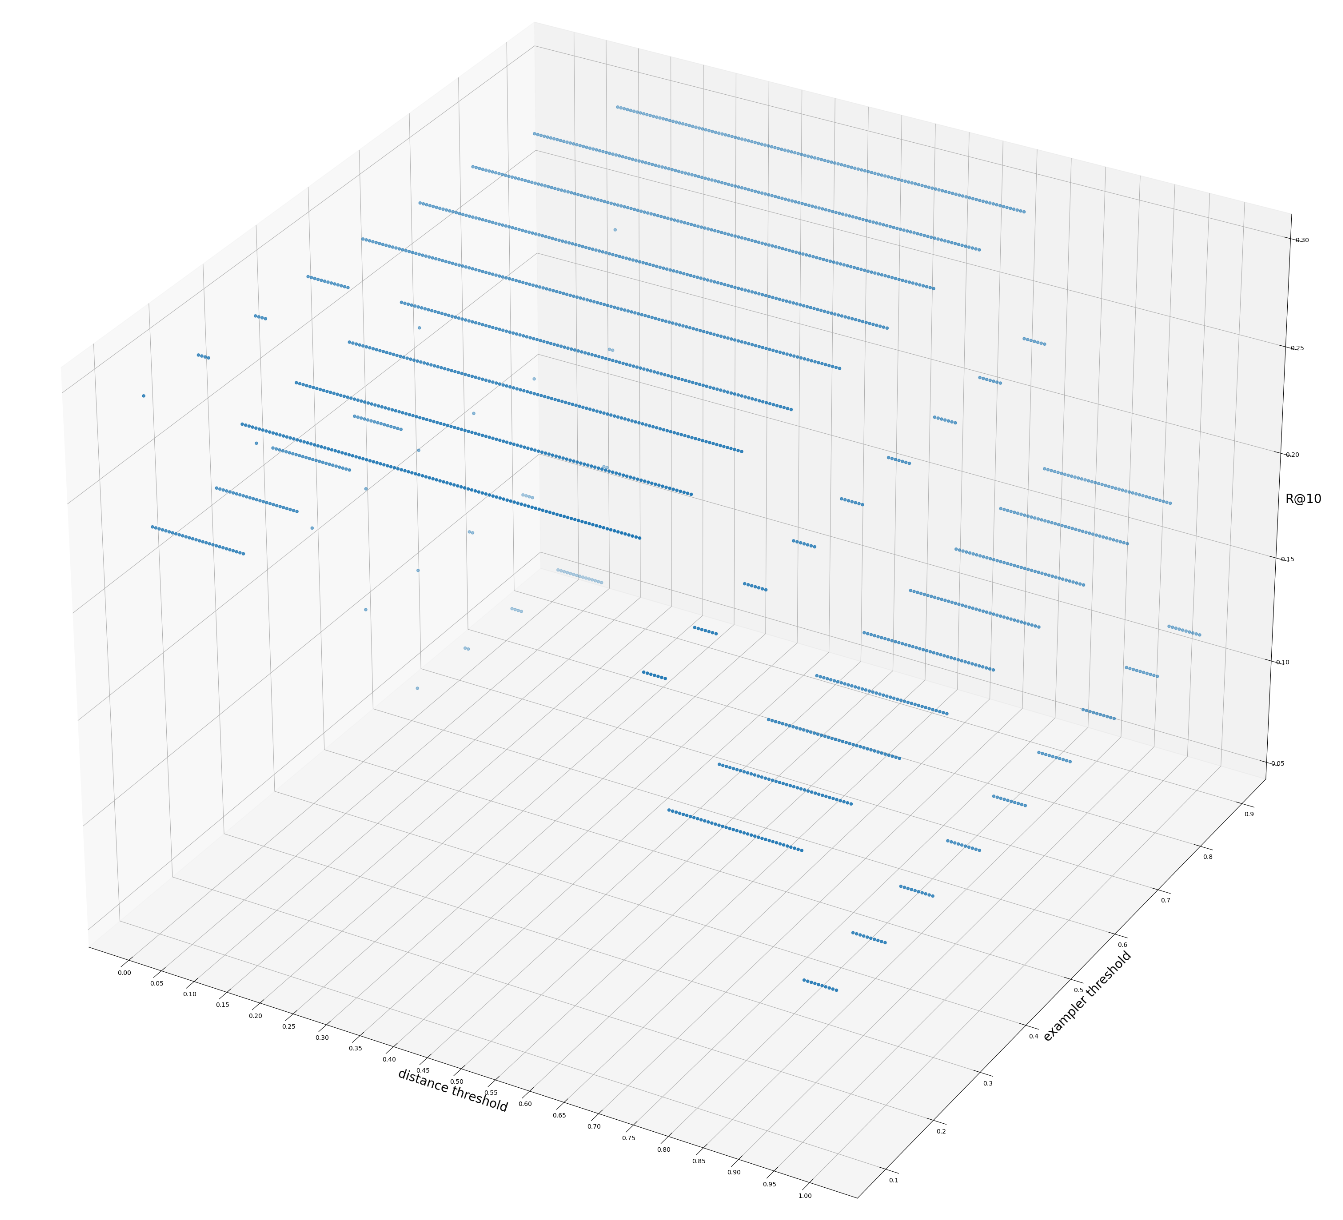
\includegraphics[width=1.0\linewidth]{r@10.png}
  \caption{阈值对R@10的影响 (Topic:Most University degrees are theoretical and do not prepare us for the real life. Do you agree or disagree)}
  \label{framework}
\end{figure*}

\begin{figure*}[htbp]\small
  \centering
  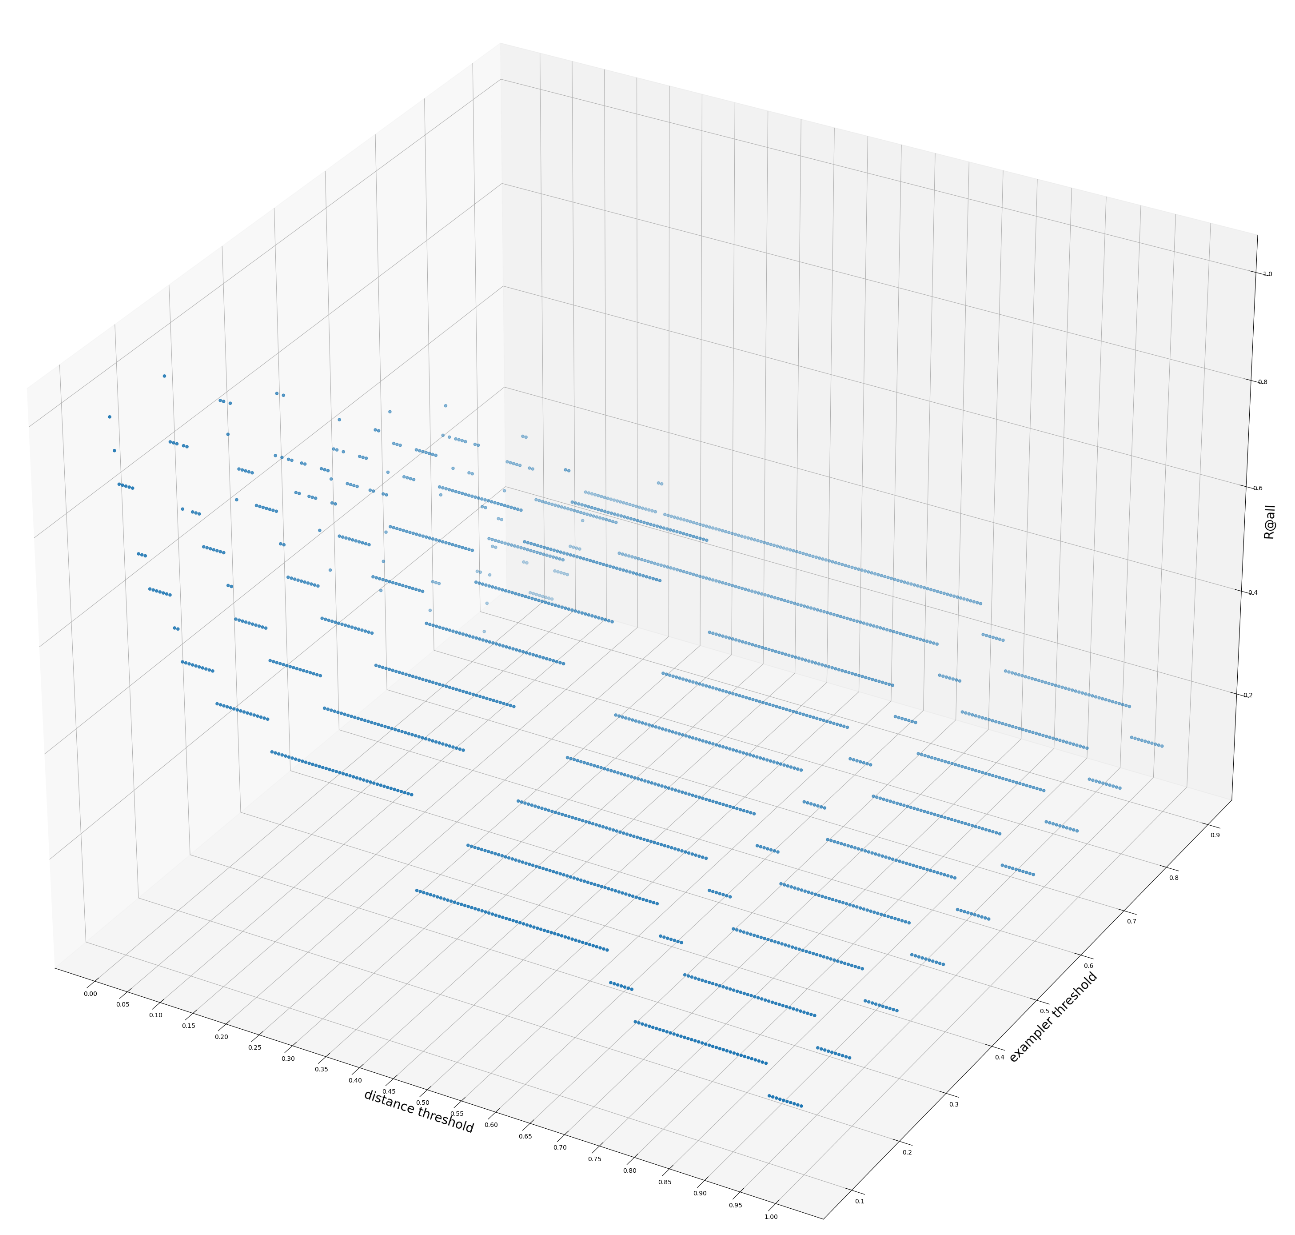
\includegraphics[width=1.0\linewidth]{r@all.png}
  \caption{阈值对R@all的影响 (Topic:Most University degrees are theoretical and do not prepare us for the real life. Do you agree or disagree)}
  \label{framework}
\end{figure*}

% Table generated by Excel2LaTeX from sheet '整理'
\begin{table}[htbp]
  \centering
  \begin{tabular}{c|c|c|c|c|c|c|c|c|c}
    \hline
    \multicolumn{2}{c}{} & \textbf{R@10} & \textbf{R@15} & \textbf{R@20} & \textbf{R@50} & \textbf{P@1} & \textbf{P@5} & \textbf{P@10} & \textbf{spearman} \\
    \hline
    \multicolumn{2}{c}{\textbf{baseline}} & 0.3917  & 0.4631  & 0.5594  & 0.7148  & 0.4545  & 0.2909  & 0.2182  & 0.1429  \\
    \hline
    \multicolumn{2}{c}{\textbf{tfidf}} & 0.4350  & 0.4533  & 0.5041  & 0.7558  & 0.4545  & 0.3091  & 0.2364  & 0.2437  \\
    \hline
    \multicolumn{2}{c}{\textbf{doc2vec}} & 0.3865  & 0.4381  & 0.5291  & 0.7041  & 0.5455  & 0.2727  & 0.2182  & 0.1865  \\
    \hline
    \multirow{2}[0]{*}{\textbf{分类模型}} & \textbf{lstm} & 0.3728  & 0.4062  & 0.4479  & 0.7398  & 0.4545  & 0.2727  & 0.1909  & 0.1535  \\
    & \textbf{bert} & 0.3029  & 0.4480  & 0.5419  & 0.7344  & 0.2727  & 0.2182  & 0.1818  & 0.0960  \\
    \hline
    \multirow{2}[0]{*}{\textbf{生成模型}} & \textbf{lstm} & 0.1263  & 0.2463  & 0.3676  & 0.7041  & 0.0000  & 0.0727  & 0.0818  & \textcolor[rgb]{ 0,  .69,  .314}{\textbf{-0.0039 }} \\
    & \textbf{bert} & \textcolor[rgb]{ 1,  0,  0}{\textbf{0.5259 }} & 0.5389  & 0.5389  & 0.7504  & 0.3636  & 0.2364  & 0.2636  & 0.1266  \\
    \hline
  \end{tabular}%
  \caption{聚类方案二(one-class)指标更新}
  \label{tab:addlabel}%
\end{table}%


% Table generated by Excel2LaTeX from sheet 'Sheet1'
\begin{table}[htbp]
  \centering
    \begin{tabular}{c|c|c|c|c|c|c|c|c|c|c}
      \hline
      \multicolumn{2}{c|}{\textcolor[rgb]{ 1,  0,  0}{}} & \textbf{R@10} & \textbf{R@15} & \textbf{R@20} & \textbf{R@50} & \textbf{R@all} & \textbf{P@1} & \textbf{P@5} & \textbf{P@10} & \textbf{spearman} \\
      \hline
      \multicolumn{2}{c|}{\textbf{baseline}} & 0.3165  & 0.3498  & 0.3552  & 0.5780  & 0.6208  & 0.1818  & 0.2364  & 0.1636  & 0.0492  \\
      \hline
      \multicolumn{2}{c|}{\textbf{tfidf}} &       &       &       &       &       &       &       &       &  \\
      \hline
      \multicolumn{2}{c|}{\textbf{doc2vec}} & 0.2528  & 0.3316  & 0.3316  & 0.6190  & 0.6404  & 0.0909  & 0.2000  & 0.1455  & 0.1257  \\
      \hline
      \multirow{2}[0]{*}{\textbf{分类模型}} & \textbf{lstm} & 0.1944  & 0.2482  & 0.2967  & 0.4090  & 0.4518  & 0.2727  & 0.1455  & 0.1182  & 0.0501  \\
      & \textbf{bert} & 0.2977  & 0.3432  & 0.4038  & 0.6017  & 0.6337  & 0.2727  & 0.2182  & 0.1818  & 0.1308  \\
      \hline
      \multirow{2}[0]{*}{\textbf{生成模型}} & \textbf{lstm} & 0.0766  & 0.1426  & 0.1715  & 0.2231  & 0.2392  & 0.0000  & 0.0545  & 0.0455  & 0.0009  \\
      & \textbf{bert} & \textcolor[rgb]{ 1,  0,  0}{\textbf{0.3873 }} & 0.4480  & 0.4533  & 0.4943  & 0.5103  & 0.2727  & 0.2545  & 0.1909  & 0.0662  \\
      \hline
    \end{tabular}%
    \begin{tablenotes}    %这行要添加, 从这开始
      \footnotesize               %这行要添加
      \item[1] R@all 表示全部小类中离题的召回
    \end{tablenotes} 
    \caption{聚类方案三(prompt-independent)指标更新}
  \label{tab:addlabel}%
\end{table}%



\end{CJK}
\end{document}

% include your own bib file like this:


%\begin{thebibliography}{}

%\bibitem[\protect\citename{Aho and Ullman}1972]{Aho:72}
%Alfred~V. Aho and Jeffrey~D. Ullman.
%\newblock 1972.
%\newblock {\em The Theory of Parsing, Translation and Compiling}, volume~1.
%\newblock Prentice-{Hall}, Englewood Cliffs, NJ.

%\bibitem[\protect\citename{{American Psychological Association}}1983]{APA:83}
%{American Psychological Association}.
%\newblock 1983.
%\newblock {\em Publications Manual}.
%\newblock American Psychological Association, Washington, DC.

%\bibitem[\protect\citename{{Association for Computing Machinery}}1983]{ACM:83}
%{Association for Computing Machinery}.
%\newblock 1983.
%\newblock {\em Computing Reviews}, 24(11):503--512.

%\bibitem[\protect\citename{Chandra \bgroup et al.\egroup }1981]{Chandra:81}
%Ashok~K. Chandra, Dexter~C. Kozen, and Larry~J. Stockmeyer.
%\newblock 1981.
%\newblock Alternation.
%\newblock {\em Journal of the Association for Computing Machinery},
%  28(1):114--133.

%\bibitem[\protect\citename{Gusfield}1997]{Gusfield:97}
%Dan Gusfield.
%\newblock 1997.
%\newblock {\em Algorithms on Strings, Trees and Sequences}.
%\newblock Cambridge University Press, Cambridge, UK.

%\bibitem[\protect\citename{Rasooli and Tetreault}2015]{rasooli-tetrault-2015}
%Mohammad~Sadegh Rasooli and Joel~R. Tetreault. 2015.
%\newblock {Yara parser: {A} fast and accurate dependency parser}.
%\newblock \emph{Computing Research Repository}, arXiv:1503.06733.
%\newblock Version 2.

%\bibitem[\protect\citename{Borschinger and Johnson}2011]{borsch2011}
%Benjamin Borschinger and Mark Johnson. 2011.
%\newblock A particle filter algorithm for {B}ayesian wordsegmentation.
%\newblock In \emph{Proceedings of the Australasian Language Technology Association %Workshop 2011}, pages 10--18, Canberra, Australia.

%\end{thebibliography}

